\documentclass[10pt]{article}

% Packages
\usepackage[margin=1in]{geometry}   % 1 inch margins
\usepackage{fancyhdr}               % Custom headers/footers
\usepackage{lastpage}               % Reference total page number
\usepackage{graphicx}
\usepackage{caption}
\usepackage{comment}
\usepackage{subcaption}
\usepackage{titlesec}
\usepackage{array}
\usepackage[most]{tcolorbox}
\usepackage{cleveref}
\usepackage{pgfgantt}
\usepackage{adjustbox} % adjust the side of the gant chart
%%%%

%% Check to see which of the below are actually needed
\usepackage{amsmath}
\usepackage{graphicx}
\usepackage{geometry}
\usepackage{amsfonts}

\usepackage{tikz}
\usetikzlibrary{arrows.meta, positioning, shapes, fit}


\newcommand\Title{Fault Tolerant Quantum Repeaters}
% 


% Expanding and Developing....

\usepackage[numbers,sort]{natbib} % Cite things in order in the body
%% Removed from the data managemnt page
%\usepackage{times}
\usepackage{url}
\usepackage{color} % needed for todo
\usepackage{enumitem}
\usepackage{soul} % highlighting 
%\setlist{leftmargin=6.0mm, noitemsep}
\setlist{noitemsep}
\usepackage{cleveref} %Cref

\usepackage{xspace} % Needed for et al.
\newcommand{\ie}{\emph{i.e.,}\xspace}
\newcommand{\eg}{\emph{e.g.,}\xspace}
\newcommand{\etc}{etc.\xspace}
\newcommand{\etal}{\emph{et~al.}\xspace} 
%\newcommand{\acite}[1]{\citeauthor{#1}~\cite{#1}} % Not working

\newlist{learningObjectives}{enumerate}{1}
%\setlist[learningObjectives, 1]{leftmargin=.7in, label = LO\arabic*:, noitemsep}
%\setlist[learningObjectives, 1]{leftmargin=.13in, noitemsep}
\setlist[learningObjectives,1]{label={},noitemsep, leftmargin=.13in}% 
\newcommand{\LearningObjective}[3]{#1: #2 (#3)}
\newcommand{\descStep}[2]{\noindent \textbf{#1: } #2}
\newcommand{\smallTitle}[1]{\vspace{1mm} \noindent \textbf{#1: }}
\newcommand{\descIStep}[2]{\noindent \emph{#1: } #2} % Italics not just bold

\newcommand{\todo}[1]{\textcolor{cyan}{\textbf{[#1]}}}
\newcommand{\dan}[1]{\textcolor{blue}{{\it [Dan: #1]}}}
\newcommand{\travis}[1]{\textcolor{green}{{\it [Travis: #1]}}}
\newcommand{\jason}[1]{\textcolor{red}{{\it [Jason: #1]}}}




%\newcommand\Title{Contextual and Uncertainty-Aware Adaptive Quantum Error Management1}
\newcommand\MainTitle{Supporting Fault-Tolerant Quantum Repeaters with Contextual and Uncertainty-Aware Adaptive Quantum Error Management}

\setlist{noitemsep, leftmargin=6.0mm}

\usepackage{tikz}
\usetikzlibrary{shapes.geometric, arrows.meta, positioning}

% Header and footer setup
\pagestyle{fancy}
\fancyhf{} % Clear all header/footer fields

% Define values for the header

\fancyhead[L]{\MainTitle}
\fancyhead[C]{}
%\fancyhead[R]{dxkvse@rit.edu}
\fancyhead[R]{XXXXXX}


% Footer: Page x of y
\fancyfoot[C]{Page \thepage\ of \pageref{lastpage}}

% Title
\title{\vspace{-2cm} \bfseries \MainTitle}%: Integrating DRL, CMAB, and Post-Processing Strategies}
%\author{Daniel Krutz \{dxkvse@rit.edu\}\\}
\author{Daniel Krutz \{dxkvse@rit.edu\}\\}

\date{}

%% Change the size of the section labels
\titleformat{\section}
  {\normalfont\bfseries\Large} % font and size %large
  {\thesection}{1em}{}              % section number formatting

%% Change the spacing between sections
\titlespacing*{\section}
  {0pt}   % Left margin
  {1ex}   % Space before the section
  {0.5ex} % Space after the section

\begin{document}

%% start defining the layout of the 1st page
\fancypagestyle{firstpage}{
  \fancyhf{}              % Clear all header/footer
  \renewcommand{\headrulewidth}{0pt} % No header rule
  \fancyfoot[C]{Page \thepage\ of \pageref{lastpage}} 
}
%% end defining the layout of the 1st page

\maketitle
%\thispagestyle{fancy} % Apply fancy header/footer to title page
%\thispagestyle{empty} % Suppress header/footer on the first page
\thispagestyle{firstpage}

\vspace{-8mm}
{\par\centering
 \begin{tcolorbox}[enhanced, width=1.03\linewidth, 
            %colback=blue!50!white!20,
            arc=0pt, outer arc=0pt, 
            borderline={1.5pt}{0pt}{black!90},
            borderline={0.25pt}{3pt}{black!70, sharp corners},
            drop fuzzy shadow]
    \centering
{\large %\textbf{Synopsis}
\par\medskip}
\normalsize%\itshape
Intelligently apply real-time/post processing error management strategies to Fault Tolerant Quantum Repeaters (FTQR) to enable effective, but resource friendly error management.
\end{tcolorbox}\par}

%%%%%%%%%%%%%%%%%%%%%%%%%%%%%%%%%%%%%%%%%%%%%%%%%%%%%%%

\section*{Overview}
Fault-tolerant quantum repeaters (FTQR) provide error-corrected, high-fidelity transmission of quantum information across long distances by continuously detecting and correcting errors during entanglement and communication processes. FTQR represent the future of quantum data networking. FTQR utilize various QEC strategies to ensure that data is correct. In traditional quantum repeaters, error correction strategies remain static and preconfigured, failing to account for temporal and spatial variations in hardware noise, photon loss, and entanglement fidelity. The current implementation of FTQR are limited by several factors including very high resource requirements, quantum memory and coherence limitations, complexity of error correction at the network scale.


The objective of this work is to support the more efficient implementation of FTQR through a more efficient and effective implementation of QEC strategies. This will be addressed through the development, implementation and evaluation of the `Adaptive Quantum Error Mitigation' (FTQR-AQEM) framework. This framework will provide dynamic, context-aware error management for fault-tolerant quantum repeaters, improving end-to-end entanglement fidelity while efficiently allocating limited qubit and computational resources. By integrating predictive modeling, adaptive QEC selection, and decentralized decision-making, it enables robust, scalable, and resource-efficient quantum communication across noisy and variable network conditions.




%%%%%%%%%%%%%%%%%%%%%%%%%%%%%%%%%%%%%%%%%%%%%%%%%%%%%%%%
%%%%%%%%%%%%%%%%%%%%%%%%%%%%%%%%%%%%%%%%%%%%%%%%%%%%%%%%
%%%%%%%%%%%%%%%%%%%%%%%%%%%%%%%%%%%%%%%%%%%%%%%%%%%%%%%%



\begin{figure}[h!]
\centering
\scalebox{0.99}{
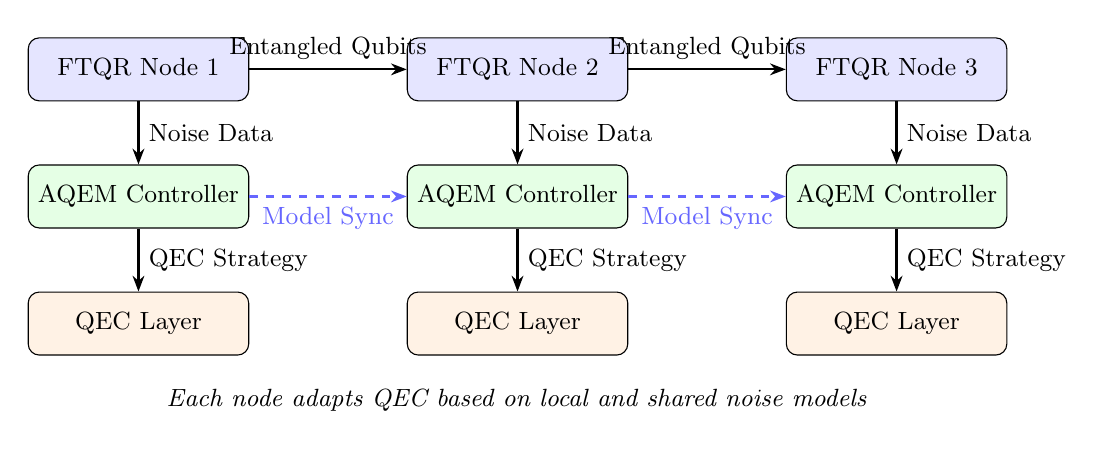
\begin{tikzpicture}[
  node distance=0.8cm and 2cm,
  box/.style={rectangle, draw, rounded corners=4pt, minimum width=2.8cm, minimum height=0.8cm, align=center},
  arrow/.style={-{Stealth[length=2mm]}, thick},
  dashedbox/.style={rectangle, dashed, draw, rounded corners=6pt, inner sep=5pt, fill=blue!2},
  every node/.style={font=\small}
]

% Nodes for Repeaters
\node[box, fill=blue!10] (R1) {FTQR Node 1};
\node[box, fill=blue!10, right=of R1] (R2) {FTQR Node 2};
\node[box, fill=blue!10, right=of R2] (R3) {FTQR Node 3};

% AQEM controllers below each
\node[box, fill=green!10, below=of R1] (A1) {AQEM Controller};
\node[box, fill=green!10, below=of R2] (A2) {AQEM Controller};
\node[box, fill=green!10, below=of R3] (A3) {AQEM Controller};

% QEC layer below AQEM
\node[box, fill=orange!10, below=of A1] (Q1) {QEC Layer};
\node[box, fill=orange!10, below=of A2] (Q2) {QEC Layer};
\node[box, fill=orange!10, below=of A3] (Q3) {QEC Layer};

% Communication arrows (Quantum channel)
\draw[arrow] (R1) -- node[above]{Entangled Qubits} (R2);
\draw[arrow] (R2) -- node[above]{Entangled Qubits} (R3);

% Vertical connections (AQEM + QEC)
\foreach \x/\y in {R1/A1, R2/A2, R3/A3} {
  \draw[arrow] (\x) -- node[right]{Noise Data} (\y);
}
\foreach \x/\y in {A1/Q1, A2/Q2, A3/Q3} {
  \draw[arrow] (\x) -- node[right]{QEC Strategy} (\y);
}

% Distributed learning connections between AQEMs
\draw[arrow, dashed, blue!60] (A1) -- node[below]{Model Sync} (A2);
\draw[arrow, dashed, blue!60] (A2) -- node[below]{Model Sync} (A3);

% Labels
\node[below=0.3cm of Q2] {\textit{Each node adapts QEC based on local and shared noise models}};

\end{tikzpicture}
}
\caption{Overview of Our Fault-Tolerant Quantum Repeater Architecture, with Each Node Supported by Our Model for QECC Selection.}
\label{fig:AQEMarchitecture}
\end{figure}


%%%%%%%%%%%%%%%%%%%%%%%%%%%%%%%%%%%%%%%%%%%%%%%%%%%%%%%%
%%%%%%%%%%%%%%%%%%%%%%%%%%%%%%%%%%%%%%%%%%%%%%%%%%%%%%%%
%%%%%%%%%%%%%%%%%%%%%%%%%%%%%%%%%%%%%%%%%%%%%%%%%%%%%%%%



%%%%%%%%%%%%%%%%%%%%%%%%%%%%%%%%%%%%%%%%%%%%%%%%%%%%%%%%%%%%
%%%%%%%%%%%%%%%%%%%%%%%%%%%%%%%%%%%%%%%%%%%%%%%%%%%%%%%%%%%%

\usetikzlibrary{fit}

\tikzstyle{arrow} = [thick,->,>=stealth]
\tikzstyle{rrec} = [rectangle, draw, fill=white!20, text width=8.95em, text centered, minimum height=2.7em]
\tikzstyle{rrecsmall} = [rectangle, draw, fill=white!20, text width=8.95em, text centered, minimum height=1.35em]
\tikzstyle{feedback} = [draw, -{Stealth[length=2mm]}, thick, dashed]
%\tikzstyle{labelnode} = [text width=8em, align=center, font=\footnotesize]
\tikzstyle{labelnode} = [text width=18em, align=center, font=\footnotesize]
\tikzstyle{dottedbox} = [draw, dashed, rounded corners, inner sep=6pt, fit=#1]

\begin{figure}[h!]
\footnotesize
\begin{center}
\scalebox{.95}{
\begin{tikzpicture}[node distance = 3.6cm, line width=.5mm]

% Main nodes
\node [rrec, minimum width=8.4em, text width=9em] (1) {Context Mapping};
\node [rrec, right of=1, minimum width=8.4em, text width=9em] (2) {Noise/Fidelity Prediction};
\node [rrec, right of=2, minimum width=8.4em, text width=9em] (3) {Adaptive Strategy Selection};
\node [rrec, right of=3, minimum width=8.4em, text width=9em] (4) {Rule Verification};
\node [rrec, right of=4, minimum width=8.4em, text width=9em] (5) {Execution \& Logging};

% Arrows
\draw [arrow] (1) -- (2);
\draw [arrow] (2) -- (3);
\draw [arrow] (3) -- (4);
\draw [arrow] (4) -- (5);

% Feedback loop
\coordinate (feedbackstart) at ($(5.south) + (0,-0.0)$);
\coordinate (feedbackmid) at ($(3.south) + (0,-0.5)$);
\coordinate (feedbackend) at ($(1.south) + (0,-0.0)$);

\draw [feedback] (feedbackstart) |- (feedbackmid) -| (feedbackend);

% Feedback label
\node [labelnode, below=0.0cm of feedbackmid, align=center] {Feedback Loop \& Continual Learning};

\end{tikzpicture}
} % end scalebox
\caption{Generalized Adaptive Error Management Framework For Run-Time/Post Processing}
\label{fig: GeneralProcess}
\end{center}
\end{figure}

%%%%%%%%%%%%%%%%%%%%%%%%%%%%%%%%%%%%%%%%%%%%%%%%%%%%%%%%%%%%
%%%%%%%%%%%%%%%%%%%%%%%%%%%%%%%%%%%%%%%%%%%%%%%%%%%%%%%%%%%%


\label{lastpage}
%\cleardoublepage


%\appendix


%% DK: Put onto a different page since it does not count against the page limit
%\setcounter{page}{1}

%\cfoot{\thepage}
%\pagenumbering{roman}
%\section{Appendix}

%\input{sections/Appendix.tex}


%% I think the appendix goes before the bib. Otherwise, I could see people missing it
%\newpage
%\pagebreak
%\addcontentsline{toc}{section}{References}
%\bibliographystyle{plain}
%\bibliography{refs}
\end{document}



